\chapter[2025 May]{May 2025}

\section[2025/03/05]{Saturday, 3 May 2025}
\label{sec:20250305}

Extend the moa timeline to be 2 years

\begin{longtable}{@{} c c p{10.5cm} @{}}
\caption{Master's Project Timeline (25 Apr 2025 -- 30 Sep 2026): Graph-Based Multiperson Pose Tracking}
\label{tab:masters-timeline-v2}\\

\toprule
\textbf{Cycle} & \textbf{Dates} & \textbf{Key goals and deliverables} \\
\midrule
\endfirsthead

\toprule
\textbf{Cycle} & \textbf{Dates} & \textbf{Key goals and deliverables} \\
\midrule
\endhead

\midrule
\multicolumn{3}{r}{\small\itshape (continued on next page)}\\
\endfoot

\bottomrule
\endlastfoot
1  & 25 Apr 2025 - 8 May 2025 & • Finalise research questions and success metrics (mAP, MOTA, ID-F1)\\
   &                & • Dockerise CUDA-enabled environment \\
   &                & • Download MS-COCO and verify checksums\\
\midrule
2  & 9 May 2025 - 22 May 2025 & • Build data-loading and augmentation pipeline for keypoints + instance masks\\
   &                & • Visual sanity-check (plot 100 annotated images)\\
   &                & • Outline baseline detector strategy\\
\midrule
3  & 23 May 2025 - 5 Jun 2025 & • Integrate lightweight depth estimator (e.g.\ MiDaS)\\
   &                & • Prototype depth-aware joint-affinity features\\
\midrule
4  & 6 Jun 2025 - 19 Jun 2025 & • Design initial Graph Attention Network (nodes = joints; edges = affinity)\\
   &                & • Implement PyTorch-Geometric \texttt{Data} objects and batching\\
\midrule
5  & 20 Jun 2025 - 3 Jul 2025 & • End-to-end prototype: detector -> depth -> GAT -> labelled poses\\
   &                & • Small-scale training for convergence/memory debugging\\
\midrule
6  & 4 Jul 2025 - 17 Jul 2025 & • Full-dataset training run; monitor loss and metrics\\
   &                & • Hyper-parameter sweep (dims, heads, depth-weight scaling)\\
\midrule
7  & 18 Jul 2025 - 31 Jul 2025 & • Consolidate training results; benchmark runtime/memory\\
   &                & • Refactor code here (will probably be needed). Good interfaces and modularity for future work.\\
\midrule
8  & 1 Aug 2025 - 14 Aug 2025 & • Implement first alternative tracker (transformer baseline)\\
   &                & • Comparative evaluation with identical metrics\\
\midrule
9  & 15 Aug 2025 - 28 Aug 2025 & • Implement second alternative tracker and benchmark\\
   &                & • Aggregate interim results and plots\\
\midrule
10 & 29 Aug 2025 - 11 Sep 2025 & • Analyse failure cases; refine affinity features/losses\\
   &                & • Prepare progress report (1 year mark; not necessarily a report) for supervisor\\
\midrule
11 & 12 Sep 2025 - 25 Sep 2025 & • Extended tuning and ablation studies\\
   &                & • Freeze model architecture for final experiments\\
\midrule
12 & 26 Sep 2025 - 9 Oct 2025 & • Re-run final experiments across validation splits\\
   &                & • Draft reproducibility checklist (README should mostly be done at this point) and code docs (docs only if not behind it will be useful)\\
\midrule
13 & 10 Oct 2025 - 23 Oct 2025 & • Add CrowdPose (or similar) for generalisation testing\\
   &                & • Cross-dataset evaluation\\
\midrule
14 & 24 Oct 2025 - 6 Nov 2025 & • Optimise inference speed (ONNX/TorchScript)\\
\midrule
15 & 7 Nov 2025 - 20 Nov 2025 & • Compile interim results to be reviewed\\
\midrule
16 & 21 Nov 2025 - 4 Dec 2025 & • Large-scale training reruns with frozen hyper-params\\
   &                & • Collect metrics and checkpoints for archiving\\
\midrule
17 & 5 Dec 2025 - 18 Dec 2025 & • Generate publish-quality figures and tables\\
\midrule
18 & 19 Dec 2025 - 1 Jan 2026 & • Codebase cleanup (holiday time this might not get done realistically)\\
\midrule
19 & 2 Jan 2026 - 15 Jan 2026 & • Robustness tests (occlusion, crowding, blur)\\
   &                & • Aggregate extra metrics (ID-switches, FPS)\\
\midrule
20 & 16 Jan 2026 - 29 Jan 2026 & • Finalise datasets/metrics\\
\midrule
21 & 30 Jan 2026 - 12 Feb 2026 & • Create overview diagram for papers\\
\midrule
22 & 13 Feb 2026 - 26 Feb 2026 & • Save data and models to be shared with reviewers who need to verify results\\
   &                & • Outline \emph{Methods} for both documents\\
\midrule
23 & 27 Feb 2026 - 12 Mar 2026 & • Final experimental pass; collect all raw outputs/images\\
   &                & • Mid-March milestone - coding phase complete\\
\midrule
24 & 13 Mar 2026 - 26 Mar 2026 & • Begin concurrent writing: detailed outlines (journal \& dissertation)\\
   &                & • Literature refresh and BibTeX management\\
\midrule
25 & 27 Mar 2026 - 9 Apr 2026 & • Draft \emph{Methods} and \emph{Experiments} (both docs)\\
   &                & • Insert key figures/tables\\
\midrule
26 & 10 Apr 2026 - 23 Apr 2026 & • Draft \emph{Results} and \emph{Discussion}\\
   &                & • Iterative revision with supervisor\\
\midrule
27 & 24 Apr 2026 - 7 May 2026 & • Draft journal \emph{Intro} \& \emph{Related Work}\\
   &                & • Populate dissertation background chapter\\
\midrule
28 & 8 May 2026 - 21 May 2026 & • Continue writing different sections\\
   &                & • Proof first half of dissertation\\
\midrule
29 & 22 May 2026 - 4 Jun 2026 & • Update citations; polish figures\\
   &                & • Journal manuscript should be mostly complete\\
\midrule
30 & 5 Jun 2026 - 18 Jun 2026 & • \textbf{Journal first draft complete} (around 15 Jun); submit to supervisor for review\\
\midrule
31 & 19 Jun 2026 - 2 Jul 2026 & • Revise journal; apply formatting; prepare cover letter\\
\midrule
32 & 3 Jul 2026 - 16 Jul 2026 & • Submit journal (pending supervisor sign-off)\\
   &                & • Draft dissertation \emph{Conclusion} \& \emph{Future Work}\\
\midrule
33 & 17 Jul 2026 - 30 Jul 2026 & • Full dissertation draft read through; integrate journal feedback\\
\midrule
34 & 31 Jul 2026 - 13 Aug 2026 & • Revise chapters; update references/appendices\\
\midrule
35 & 14 Aug 2026 - 27 Aug 2026 & • \textbf{Dissertation first draft finalised} (31 Aug); send for review\\
\midrule
36 & 28 Aug 2026 - 10 Sep 2026 & • Address feedback\\
   &                & • Full LaTeX proof (lists, glossaries, links)\\
\midrule
37 & 11 Sep 2026 - 24 Sep 2026 & • \textbf{Final dissertation draft complete} (30 Sep)\\
   &                & • Supervisor sign-off; prepare submission\\
\midrule
38 & 25 Sep 2026 - 8 Oct 2026 & • Submit final dissertation and whatever else is required like code and models\\
\end{longtable}

\section[2025/23/05]{Saturday, 23 May 2025}
\label{sec:20252305}

I've been really bad with commiting there are a number of changes I've made.

I'm going to continue on basic on what I'm doing and add some detailed notes
(made notes in another directory but will include them here)

\subsection{Initial Setup}

The most basic experiment using the code at this date. The main file is given as

\begin{lstlisting}[style=pythonstyle,title={Main file for initial setup May},label={code:init}]
import matplotlib
matplotlib.use('TkAgg')
from dataloader import create_coco_dataloader
from test import test_dataloader, test_depth_estimator, test_keypoint_rcnn
from utils import process_single_image, build_graph_features, process_batch
import numpy as np
from gat import prepare_dataset, train_gat
from settings import settings
import torch

def main():
    dataloader = create_coco_dataloader(
        split='train', 
        batch_size=4
    )
    
    # test_dataloader(dataloader)
    # test_depth_estimator(dataloader)
    # test_keypoint_rcnn(dataloader)
    
    print("Extracting features from images...")
    all_node_features = process_batch(dataloader, num_batches=10)
    print(f"Extracted features for {len(all_node_features)} people")
    
    if len(all_node_features) > 0:
        print("\nPreparing dataset for GAT training...")
        dataset = prepare_dataset(all_node_features)
        
        print("\nTraining GAT model...")
        model = train_gat(dataset, epochs=150)
        
        model_path = f"{settings.output_dir}/pose_gat_model.pt"
        torch.save(model.state_dict(), model_path)
        print(f"Model saved to {model_path}")
    else:
        print("No valid features extracted. Cannot train GAT model.")
    
if __name__ == "__main__":
    main()
\end{lstlisting}

The output is as follows

Part 1 is the results of batch processing and looks something like this I just chose a batch at random in this case batch 3

\begin{lstlisting}[style=bashstyle,title={Initial output of batch processing},label={code:init_batch_processing}]
Processing batch 3/10
  Processing image 1/4 (ID: 36006)
Using cache found in /home/dean/.cache/torch/hub/intel-isl_MiDaS_master
Loading weights:  None
Using cache found in /home/dean/.cache/torch/hub/rwightman_gen-efficientnet-pytorch_master
Found 2 people in image 36006
  Processing image 2/4 (ID: 334019)
Using cache found in /home/dean/.cache/torch/hub/intel-isl_MiDaS_master
Loading weights:  None
Using cache found in /home/dean/.cache/torch/hub/rwightman_gen-efficientnet-pytorch_master
Found 4 people in image 334019
  Processing image 3/4 (ID: 138656)
Using cache found in /home/dean/.cache/torch/hub/intel-isl_MiDaS_master
Loading weights:  None
Using cache found in /home/dean/.cache/torch/hub/rwightman_gen-efficientnet-pytorch_master
Found 1 people in image 138656
  Processing image 4/4 (ID: 343038)
Using cache found in /home/dean/.cache/torch/hub/intel-isl_MiDaS_master
Loading weights:  None
Using cache found in /home/dean/.cache/torch/hub/rwightman_gen-efficientnet-pytorch_master
Found 13 people in image 343038
Processing batch 4/10
  Processing image 1/4 (ID: 540740)
Using cache found in /home/dean/.cache/torch/hub/intel-isl_MiDaS_master
Loading weights:  None
Using cache found in /home/dean/.cache/torch/hub/rwightman_gen-efficientnet-pytorch_master
Found 8 people in image 540740
  Processing image 2/4 (ID: 277746)
Using cache found in /home/dean/.cache/torch/hub/intel-isl_MiDaS_master
Loading weights:  None
Using cache found in /home/dean/.cache/torch/hub/rwightman_gen-efficientnet-pytorch_master
Found 1 people in image 277746
  Processing image 3/4 (ID: 111142)
Using cache found in /home/dean/.cache/torch/hub/intel-isl_MiDaS_master
Loading weights:  None
Using cache found in /home/dean/.cache/torch/hub/rwightman_gen-efficientnet-pytorch_master
Found 2 people in image 111142
  Processing image 4/4 (ID: 41231)
Using cache found in /home/dean/.cache/torch/hub/intel-isl_MiDaS_master
Loading weights:  None
Using cache found in /home/dean/.cache/torch/hub/rwightman_gen-efficientnet-pytorch_master
Found 10 people in image 41231
\end{lstlisting}

The second part (the results) look like this

\begin{lstlisting}[style=bashstyle,title={Initial output of results},label={code:init_batch_results}]
Training GAT model...
/home/dean/projects/mills_ds/.venv/lib/python3.12/site-packages/torch_geometric/deprecation.py:26: UserWarning: 'data.DataLoader' is deprecated, use 'loader.DataLoader' instead
  warnings.warn(out)
Epoch 010, Loss: 643.0189
Epoch 020, Loss: 584.6199
Epoch 030, Loss: 617.5257
Epoch 040, Loss: 615.4443
Epoch 050, Loss: 620.4097
Epoch 060, Loss: 607.3152
Epoch 070, Loss: 546.9651
Epoch 080, Loss: 555.2163
Epoch 090, Loss: 576.3951
Epoch 100, Loss: 532.3719
Epoch 110, Loss: 510.0810
Epoch 120, Loss: 586.6923
Epoch 130, Loss: 516.5629
Epoch 140, Loss: 486.8763
Epoch 150, Loss: 492.9085
\end{lstlisting}

\todoredefined{There is a bug in the code and using more than 20 batches causes exceptions. Will need to fix that}
A further example where $num\_batches = 20$ and $epochs = 300$
this is the output

\begin{lstlisting}[style=bashstyle,title={Initial output of results with larger batch and epochs},label={code:init_batch_results_1}]
Epoch 010, Loss: 1026.5993
Epoch 020, Loss: 1071.3685
Epoch 030, Loss: 947.4141
Epoch 040, Loss: 972.9103
Epoch 050, Loss: 944.9288
Epoch 060, Loss: 967.7079
Epoch 070, Loss: 1050.1810
Epoch 080, Loss: 967.5399
Epoch 090, Loss: 904.2044
Epoch 100, Loss: 908.0457
Epoch 110, Loss: 890.5145
Epoch 120, Loss: 942.8686
Epoch 130, Loss: 851.8860
Epoch 140, Loss: 856.3290
Epoch 150, Loss: 813.2121
Epoch 160, Loss: 846.5770
Epoch 170, Loss: 826.4389
Epoch 180, Loss: 847.7061
Epoch 190, Loss: 818.5656
Epoch 200, Loss: 833.8501
Epoch 210, Loss: 827.2758
Epoch 220, Loss: 818.5506
Epoch 230, Loss: 764.1811
Epoch 240, Loss: 777.7470
Epoch 250, Loss: 756.4544
Epoch 260, Loss: 749.1353
Epoch 270, Loss: 782.7563
Epoch 280, Loss: 818.9373
Epoch 290, Loss: 756.4029
Epoch 300, Loss: 725.9068
\end{lstlisting}

The idea here is that the model is trianed and the loss is decreasing at least
in some capacity. It's no where close to being done though this is just the
very first step

\subsection{Basic}

Starting with a new main file which will load the data. This is the first
actual attempt at this and I've tried to document this with some amount of
care.

\begin{lstlisting}[style=pythonstyle,title={Main file basic setup May},label={code:basic}]
import torch
import torch.nn as nn
from torch.utils.data import DataLoader
import numpy as np
from tqdm import tqdm

from dataloader import create_coco_dataloader
from dataset import CocoKeypointsDataset
from settings import settings

def main():
    # Set device
    device = torch.device('cuda' if torch.cuda.is_available() else 'cpu')
    print(f"Using device: {device}")
    
    # Hyperparameters
    batch_size = 4
    num_epochs = 10
    learning_rate = 1e-4
    
    # Create dataloaders
    print("Loading datasets...")
    train_loader = create_coco_dataloader(
        split='train',
        batch_size=batch_size,
        shuffle=True,
        num_workers=2
    )
    
    val_loader = create_coco_dataloader(
        split='val',
        batch_size=batch_size,
        shuffle=False,
        num_workers=2
    )
    
    print(f"Train samples: {len(train_loader.dataset)}")
    print(f"Val samples: {len(val_loader.dataset)}")
    
    # Test loading a batch
    print("\nTesting data loading...")
    for i, batch in enumerate(train_loader):
        print(f"\nBatch {i}:")
        print(f"  Images: {len(batch['image'])} images")
        print(f"  Image shapes: {[img.shape for img in batch['image']]}")
        print(f"  Keypoints per image: {[len(kps) for kps in batch['keypoints']]}")
        
        # Check first image's keypoints
        if len(batch['keypoints'][0]) > 0:
            print(f"  First person keypoints shape: {batch['keypoints'][0][0].shape}")
        
        if i >= 2:
            break
    
    print("\nData loading successful!")

if __name__ == "__main__":
    main()
\end{lstlisting}

The output of this will look something like this:

\begin{lstlisting}[style=bashstyle,title={Main file basic output},label={code:basic_output}]
Using device: cuda
Loading datasets...
loading annotations into memory...
Done (t=2.21s)
creating index...
index created!
Loaded 64115 images with person keypoints
loading annotations into memory...
Done (t=0.09s)
creating index...
index created!
Loaded 2693 images with person keypoints
Train samples: 64115
Val samples: 2693

Testing data loading...

Batch 0:
  Images: 4 images
  Image shapes: [torch.Size([3, 427, 640]), torch.Size([3, 427, 640]), torch.Size([3, 480, 640]), torch.Size([3, 465, 640])]
  Keypoints per image: [5, 2, 5, 1]
  First person keypoints shape: torch.Size([17, 3])

Batch 1:
  Images: 4 images
  Image shapes: [torch.Size([3, 500, 375]), torch.Size([3, 427, 640]), torch.Size([3, 429, 640]), torch.Size([3, 334, 500])]
  Keypoints per image: [2, 5, 1, 1]
  First person keypoints shape: torch.Size([17, 3])

Batch 2:
  Images: 4 images
  Image shapes: [torch.Size([3, 426, 640]), torch.Size([3, 427, 640]), torch.Size([3, 375, 500]), torch.Size([3, 427, 640])]
  Keypoints per image: [14, 8, 5, 11]
  First person keypoints shape: torch.Size([17, 3])

Data loading successful!
\end{lstlisting}

\todoredefined{There is a bit of a problem with the wrapping here will need to figure that out at some point}

To quickly summarize this the above output \ref{code:basic_output}:
\begin{compactitem}
   \item there are 4 images per batch
   \item each image is a tensor $[3,H,W]$
      \begin{compactitem}
         \item 3 for the rgb
         \item H and W are the height and width respectively   
      \end{compactitem}
   \item keypoints per image mean how many people in each image so $[5,2,5,1]$
      \begin{compactitem}
         \item First image has 5 people detected
         \item Second image has 2 people detected
         \item Third image has 5 people detected
         \item Fourth image has 1 person detected
      \end{compactitem}
   \item Person keypoints shape $[17,3]$

      \begin{compactitem}
         \item 17 keypoints (joints) in the coco format
         \item 3 = [x,y,visibility] for each keypoint where visibility:
            \begin{compactitem}
               \item 0 = not labeled
               \item 1 = labeled but not visible
               \item 2 = labeled and visible
            \end{compactitem}
      \end{compactitem}
\end{compactitem}

This is the basic loading of the data done and the first step in the process, however,
while this serves mostly as an explination of how this works the data loader is not 100\% correct

\subsection{Preprocessing}

The next step is to do the preprocessing of the data there are three main
sections each will be briefly discussed: 

\begin{compactitem}
\item extract node features 
\item create adjacency matrix 
\item process batch
\end{compactitem}

The entire file is given below and then it will be broken up and explained in detail.
This is the first iteration of the preprocessing and the idea here is to understand
exactly whats going on

\begin{lstlisting}[style=pythonstyle,title={Preprocessing May},label={code:preprocessing_may}]
import torch
import torch.nn as nn
import numpy as np
from depth_estimation import estimate_depth

# For reference
COCO_KEYPOINT_NAMES = [
    'nose', 'left_eye', 'right_eye', 'left_ear', 'right_ear',
    'left_shoulder', 'right_shoulder', 'left_elbow', 'right_elbow',
    'left_wrist', 'right_wrist', 'left_hip', 'right_hip',
    'left_knee', 'right_knee', 'left_ankle', 'right_ankle'
]

# Define skeleton connections
SKELETON_CONNECTIONS = [
    (0, 1), (0, 2),# nose to eyes
    (1, 3), (2, 4),# eyes to ears
    (5, 7), (7, 9),# left shoulder to left elbow to left wrist
    (6, 8), (8, 10),# right shoulder to right elbow to right wrist
    (5, 6), (5, 11), (6, 12),# shoulders to hips
    (11, 13), (13, 15),# left hip to left knee to left ankle
    (12, 14), (14, 16)# right hip to right knee to right ankle
]

class KeypointPreprocessor:
    def __init__(self, num_keypoint_types=17, embedding_dim=32, device='cuda'):
        """
        Initialize the preprocessor with learnable joint-type embeddings.
        
        Args:
            num_keypoint_types: Number of different keypoint types (17 for COCO)
            embedding_dim: Dimension of the joint-type embeddings
            device: Device to use for computations
        """
        self.device = device
        self.num_keypoint_types = num_keypoint_types
        self.embedding_dim = embedding_dim
        
        # Create learnable joint-type embeddings
        self.joint_embeddings = nn.Embedding(num_keypoint_types, embedding_dim)
        self.joint_embeddings.to(device)
    
    def extract_node_features(self, image, keypoints_list, min_confidence=0.0):
        """
        Extract node features from an image and its keypoints.
        
        Args:
            image: Image tensor [C, H, W]
            keypoints_list: List of keypoint tensors, each [17, 3] for each person
            min_confidence: Minimum visibility score to include a keypoint
            
        Returns:
            node_features: Tensor of shape [N, 4 + embedding_dim] where N is total valid keypoints
            node_info: List of tuples (person_idx, keypoint_idx) for tracking
        """
        # Move image to device
        image = image.to(self.device)
        
        # Estimate depth map
        depth_map = estimate_depth(image)  # [H, W]
        
        # Collect all valid keypoints
        nodes = []
        node_info = []
        
        for person_idx, keypoints in enumerate(keypoints_list):
            # keypoints shape: [17, 3] where 3 = [x, y, visibility]
            for kp_idx in range(keypoints.shape[0]):
                x, y, visibility = keypoints[kp_idx]
                
                # Skip keypoints with low visibility
                if visibility <= min_confidence:
                    continue
                
                # Get depth value at keypoint location
                # Ensure coordinates are within bounds
                h, w = depth_map.shape
                x_int = int(torch.clamp(x, 0, w-1))
                y_int = int(torch.clamp(y, 0, h-1))
                
                depth_value = depth_map[y_int, x_int].item()
                
                # Use visibility as confidence (normalize to 0-1 range)
                # visibility: 0=not labeled, 1=occluded, 2=visible
                confidence = visibility / 2.0
                
                # Create node features [x, y, d, c]
                node_feat = torch.tensor([x.item(), y.item(), depth_value, confidence], 
                                        dtype=torch.float32, device=self.device)
                
                nodes.append(node_feat)
                node_info.append((person_idx, kp_idx))
        
        if len(nodes) == 0:
            # Return empty tensors if no valid keypoints
            return torch.zeros((0, 4 + self.embedding_dim), device=self.device), []
        
        # Stack node features
        node_features = torch.stack(nodes)  # [N, 4]
        
        # Add joint-type embeddings
        joint_types = torch.tensor([info[1] for info in node_info], 
                                  dtype=torch.long, device=self.device)
        embeddings = self.joint_embeddings(joint_types)  # [N, embedding_dim]
        
        # Concatenate basic features with embeddings
        node_features = torch.cat([node_features, embeddings], dim=1)  # [N, 4 + embedding_dim]
        
        return node_features, node_info
    
    def create_adjacency_matrix(self, node_info, num_nodes):
        """
        Create adjacency matrix based on skeleton connections.
        
        Args:
            node_info: List of tuples (person_idx, keypoint_idx)
            num_nodes: Total number of nodes
            
        Returns:
            adj_matrix: Adjacency matrix [num_nodes, num_nodes]
        """
        adj_matrix = torch.zeros((num_nodes, num_nodes), device=self.device)
        
        # Create a mapping from (person_idx, keypoint_idx) to node index
        info_to_node_idx = {info: idx for idx, info in enumerate(node_info)}
        
        # Add edges based on skeleton connections
        for (p1_idx, kp1_idx), node1_idx in info_to_node_idx.items():
            for (p2_idx, kp2_idx), node2_idx in info_to_node_idx.items():
                # Only connect keypoints from the same person
                if p1_idx != p2_idx:
                    continue
                
                # Check if these keypoints are connected in the skeleton
                if (kp1_idx, kp2_idx) in SKELETON_CONNECTIONS or \
                   (kp2_idx, kp1_idx) in SKELETON_CONNECTIONS:
                    adj_matrix[node1_idx, node2_idx] = 1.0
                    adj_matrix[node2_idx, node1_idx] = 1.0
        
        return adj_matrix
    
    def process_batch(self, batch):
        """
        Process a batch of data into graph format.
        
        Args:
            batch: Dictionary with 'image' and 'keypoints' from dataloader
            
        Returns:
            graphs: List of graph data dictionaries, one per image
        """
        images = batch['image']
        keypoints_batch = batch['keypoints']
        
        graphs = []
        
        for img_idx, (image, keypoints_list) in enumerate(zip(images, keypoints_batch)):
            # Extract node features
            node_features, node_info = self.extract_node_features(image, keypoints_list)
            
            # Skip if no valid nodes
            if len(node_info) == 0:
                continue
            
            # Create adjacency matrix
            num_nodes = node_features.shape[0]
            adj_matrix = self.create_adjacency_matrix(node_info, num_nodes)
            
            # Create graph data dictionary
            graph_data = {
                'node_features': node_features,  # [N, 4 + embedding_dim]
                'adjacency': adj_matrix,  # [N, N]
                'node_info': node_info,  # List of (person_idx, keypoint_idx)
                'image_idx': img_idx,
                'img_id': batch['img_id'][img_idx],
                'num_nodes': num_nodes,
                'num_people': len(keypoints_list)
            }
            
            graphs.append(graph_data)
        
        return graphs
\end{lstlisting}

So the init of this class


\begin{lstlisting}[style=pythonstyle,title={Preprocessing May init},label={code:preprocessing_may_init}]
    def __init__(self, num_keypoint_types=17, embedding_dim=32, device='cuda'):
        """
        Initialize the preprocessor with learnable joint-type embeddings.
        
        Args:
            num_keypoint_types: Number of different keypoint types (17 for COCO)
            embedding_dim: Dimension of the joint-type embeddings
            device: Device to use for computations
        """
        self.device = device
        self.num_keypoint_types = num_keypoint_types
        self.embedding_dim = embedding_dim
        
        # Create learnable joint-type embeddings
        self.joint_embeddings = nn.Embedding(num_keypoint_types, embedding_dim)
        self.joint_embeddings.to(device)
\end{lstlisting}

This can be described like this:

\begin{compactitem}
   \item device: Specifies GPU ('cuda') or CPU for computations
   \item num\_keypoint\_types: 17 different joint types in COCO (nose, eyes, shoulders, etc.)
   \item embedding\_dim: Size of learned representation for each joint type (default: 32)
   \item joint\_embeddings: A learnable lookup table for joint types
\end{compactitem}

\todoredefined{Thinking about this now while writing this but it's pretty dumb
to have num\_keypoint\_types since it has to be 17 for COCO. 
This will need to be improved upon later.}

The device and num\_keypoint\_types are quite obvious but the embedding\_dim and joint\_embeddings aren't

You can think of joint embeddings:

\begin{compactitem}
   \item Without embeddings: Joint type = just a number (0 for nose, 1 for left eye, etc.)
   \item With embeddings: Joint type = a rich 32-dimensional vector that captures meaning
\end{compactitem}


An analogy (for later) it's like the difference between:

\begin{compactitem}
   \item Describing a person with just their ID number (boring, limited)
   \item Describing a person with 32 characteristics (height, personality, skills, etc.)
\end{compactitem}

The underlying idea is that the network learns these rich embeddings during training and discovers patterns:
\begin{compactitem}
   \item "left shoulder" and "right shoulder" should have similar embeddings
   \item "ankle" and "wrist" might share some characteristics (both are extremities)
   \item "nose" might be quite different from limb joints
\end{compactitem}

\subsubsection{Extract Node Features}

The extract node features function is given below

\begin{lstlisting}[style=pythonstyle,title={Preprocessing May Extract Node Features},label={code:preprocessing_may_extract_node_features}]
def extract_node_features(self, image, keypoints_list, min_confidence=0.0):
   """
   Extract node features from an image and its keypoints.
   
   Args:
      image: Image tensor [C, H, W]
      keypoints_list: List of keypoint tensors, each [17, 3] for each person
      min_confidence: Minimum visibility score to include a keypoint
      
   Returns:
      node_features: Tensor of shape [N, 4 + embedding_dim] where N is total valid keypoints
      node_info: List of tuples (person_idx, keypoint_idx) for tracking
   """
   # Move image to device
   image = image.to(self.device)
   
   # Estimate depth map
   depth_map = estimate_depth(image)  # [H, W]
   
   # Collect all valid keypoints
   nodes = []
   node_info = []
   
   for person_idx, keypoints in enumerate(keypoints_list):
      # keypoints shape: [17, 3] where 3 = [x, y, visibility]
      for kp_idx in range(keypoints.shape[0]):
            x, y, visibility = keypoints[kp_idx]
            
            # Skip keypoints with low visibility
            if visibility <= min_confidence:
               continue
            
            # Get depth value at keypoint location
            # Ensure coordinates are within bounds
            h, w = depth_map.shape
            x_int = int(torch.clamp(x, 0, w-1))
            y_int = int(torch.clamp(y, 0, h-1))
            
            depth_value = depth_map[y_int, x_int].item()
            
            # Use visibility as confidence (normalize to 0-1 range)
            # visibility: 0=not labeled, 1=occluded, 2=visible
            confidence = visibility / 2.0
            
            # Create node features [x, y, d, c]
            node_feat = torch.tensor([x.item(), y.item(), depth_value, confidence], 
                                    dtype=torch.float32, device=self.device)
            
            nodes.append(node_feat)
            node_info.append((person_idx, kp_idx))
   
   if len(nodes) == 0:
      # Return empty tensors if no valid keypoints
      return torch.zeros((0, 4 + self.embedding_dim), device=self.device), []
   
   # Stack node features
   node_features = torch.stack(nodes)  # [N, 4]
   
   # Add joint-type embeddings
   joint_types = torch.tensor([info[1] for info in node_info], 
                              dtype=torch.long, device=self.device)
   embeddings = self.joint_embeddings(joint_types)  # [N, embedding_dim]
   
   # Concatenate basic features with embeddings
   node_features = torch.cat([node_features, embeddings], dim=1)  # [N, 4 + embedding_dim]
   
   return node_features, node_info
\end{lstlisting}

This function \ref{code:preprocessing_may_extract_node_features} takes in:
\begin{compactitem}
   \item an image $[C,H,W]$ 
   \item keypoint list (list of tensors $[17,3]$, one per person)
   \item min\_confidence threshold for including keypoints
\end{compactitem}

Again each tensor has 3 values $[x,y,visibility]$. node\_info keeps track of
each node comes from (person\_id,joint\_id) = (which person, which joint)

An example of this to futher illustrate node\_info:
\begin{compactitem}
   \item $(0,5)$ = person 0's left shoulder
   \item $(2,0)$ = person 2's nose
\end{compactitem}

so which person each node belongs to (for adjacency) and which joint type it is

Example:

Imagine image with 2 people:

Person 0: Only nose and left and right shoulder visible (3 keypoints above threshold)

Person 1: Only right are so right shoulder, right elbow and right writs (3 keypoints above threshold)

There will therefore be 6 nodes $node\_info = [(0,0), (0,5), (0,6), (1,6), (1,8), (1,10)]$

\begin{compactitem}
   \item Person 0's nose, left shoulder, right shoulder
   \item Person 1's right shoulder, right elbow, right wrist
\end{compactitem}

node\_features $[6,36]$ (6 nodes x (4 basic + 32 embedding))

the node\_feature contains:

\begin{compactitem}
   \item x: x coordinate in image
   \item y: y coordinate in image
   \item depth: depth value from MiDaS
   \item confidence: visibility score (0-1)
   \item 32-dim embedding: the learned representation for that joint type
\end{compactitem}

The joint types are used to get the joint embeddings (The joints types here are extracted from the example above)

\begin{lstlisting}[style=pythonstyle,title={Preprocessing May get embeddings},label={code:preprocessing_may_get_embeddings}]
joint_types = [0, 5, 6, 6, 8, 10]  # Extracted from node_info
embeddings = self.joint_embeddings(joint_types)  # Look up each joint's embedding
\end{lstlisting}

\subsubsection{Building the Adjacency Matrix}

This is the code for building the adjacency matrix

\begin{lstlisting}[style=pythonstyle,title={Preprocessing May Adjacency},label={code:preprocessing_may_adjacency_matrix}]
def create_adjacency_matrix(self, node_info, num_nodes):
   """
   Create adjacency matrix based on skeleton connections.
   
   Args:
      node_info: List of tuples (person_idx, keypoint_idx)
      num_nodes: Total number of nodes
      
   Returns:
      adj_matrix: Adjacency matrix [num_nodes, num_nodes]
   """
   adj_matrix = torch.zeros((num_nodes, num_nodes), device=self.device)
   
   # Create a mapping from (person_idx, keypoint_idx) to node index
   info_to_node_idx = {info: idx for idx, info in enumerate(node_info)}
   
   # Add edges based on skeleton connections
   for (p1_idx, kp1_idx), node1_idx in info_to_node_idx.items():
      for (p2_idx, kp2_idx), node2_idx in info_to_node_idx.items():
            # Only connect keypoints from the same person
            if p1_idx != p2_idx:
               continue
            
            # Check if these keypoints are connected in the skeleton
            if (kp1_idx, kp2_idx) in SKELETON_CONNECTIONS or \
               (kp2_idx, kp1_idx) in SKELETON_CONNECTIONS:
               adj_matrix[node1_idx, node2_idx] = 1.0
               adj_matrix[node2_idx, node1_idx] = 1.0
   
   return adj_matrix
\end{lstlisting}

This adjacency matrix is a square matrix which nodes are connected in the graph

It's a square matrix where:

\begin{compactitem}
   \item Rows = nodes
   \item columns = nodes
   \item Value 1 = connected
   \item Value 0 = not connected
\end{compactitem}

The following rules are applied:

\begin{compactitem}
   \item Only connect keypoints from same person
   \item Use COCO skeleton structure
   \item Bidirectional Connection (A connects to B, B connects to A)
\end{compactitem}

An example where you have 2 people in an image: 
\begin{compactitem}
   \item Person 0: Has 3 visible keypoints - nose (0), left shoulder (5), left elbow (7)
   \item Person 1: Has 2 visible keypoints - right shoulder (6), right elbow (8)
\end{compactitem}

The nodes would then be: 
\begin{compactitem}
\item Node 0: Person 0's nose
\item Node 1: Person 0's left shoulder
\item Node 2: Person 0's left elbow
\item Node 3: Person 1's right shoulder
\item Node 4: Person 1's right elbow
\end{compactitem}

Building the Adjacency Matrix

The COCO skeleton connections include:
\begin{compactitem}
   \item (5, 7): left shoulder <-> left elbow
   \item (6, 8): right shoulder <-> right elbow
   \item (0, 1): nose <-> left eye (but left eye not visible)
   \item etc
\end{compactitem}

\begin{table}[H]
\centering
\caption{Adjacency matrix of selected keypoints showing person-specific limb connections.}
\begin{tabular}{c|ccccc@{\hskip 1em}|@{\hskip 1em}l}
     & N0 & N1 & N2 & N3 & N4 & Description \\
\hline
N0 & 0  & 0  & 0  & 0  & 0  & Person 0's nose -- no connections \\
N1 & 0  & 0  & 1  & 0  & 0  & Person 0's left shoulder -- connects to left elbow \\
N2 & 0  & 1  & 0  & 0  & 0  & Person 0's left elbow -- connects to left shoulder \\
N3 & 0  & 0  & 0  & 0  & 1  & Person 1's right shoulder -- connects to right elbow \\
N4 & 0  & 0  & 0  & 1  & 0  & Person 1's right elbow -- connects to right shoulder \\
\end{tabular}
\label{tab:keypoint_adjacency}
\end{table}

This structure is for the following:
\begin{compactitem}
   \item No cross-person connections: Person 0's joints don't connect to Person 1's joints
   \item Anatomically meaningful: only connect joints that are physically connected in the body
   \item Symmetric: If A->B exists, then B->A exists (undirected graph)
\end{compactitem}

The GAT will use this adjacency matrix to:
\begin{compactitem}
   \item Know which nodes to attend to (connected neighbors)
   \item Aggregate information along the skeleton structure
   \item Learn relationships between connected body parts
   \item Keep different people's poses separate
\end{compactitem}

This is the main file used to test preprocessing

\begin{lstlisting}[style=pythonstyle,title={Preprocessing May Main},label={code:preprocessing_may_main}]
import torch
import torch.nn as nn
from torch.utils.data import DataLoader
import numpy as np
from tqdm import tqdm

from dataloader import create_coco_dataloader
from dataset import CocoKeypointsDataset
from settings import settings
from basic.preprocess import KeypointPreprocessor

def main():
    # Set device
    device = torch.device('cuda' if torch.cuda.is_available() else 'cpu')
    print(f"Using device: {device}")
    
    # Hyperparameters
    batch_size = 4
    num_epochs = 10
    learning_rate = 1e-4
    
    # Create dataloaders
    print("Loading datasets...")
    train_loader = create_coco_dataloader(
        split='train',
        batch_size=batch_size,
        shuffle=True,
        num_workers=2
    )
    
    val_loader = create_coco_dataloader(
        split='val',
        batch_size=batch_size,
        shuffle=False,
        num_workers=2
    )
    
    print(f"Train samples: {len(train_loader.dataset)}")
    print(f"Val samples: {len(val_loader.dataset)}")
    
    # Test loading a batch
    print("\nTesting data loading...")
    for i, batch in enumerate(train_loader):
        print(f"\nBatch {i}:")
        print(f"  Images: {len(batch['image'])} images")
        print(f"  Image shapes: {[img.shape for img in batch['image']]}")
        print(f"  Keypoints per image: {[len(kps) for kps in batch['keypoints']]}")
        
        # Check first image's keypoints
        if len(batch['keypoints'][0]) > 0:
            print(f"  First person keypoints shape: {batch['keypoints'][0][0].shape}")
        
        if i >= 2:  # Just check first 3 batches
            break
    
    print("\nData loading successful!")
    
    # Test preprocessing
    print("\n" + "="*50)
    print("Testing preprocessing...")
    preprocessor = KeypointPreprocessor(device=device)
    
    # Get one batch for testing
    for batch in train_loader:
        graphs = preprocessor.process_batch(batch)
        
        print(f"\nProcessed {len(graphs)} graphs from batch of {len(batch['image'])} images")
        
        for i, graph in enumerate(graphs[:3]):  # Show first 3 graphs
            print(f"\nGraph {i}:")
            print(f"  Image ID: {graph['img_id']}")
            print(f"  Number of people: {graph['num_people']}")
            print(f"  Number of nodes: {graph['num_nodes']}")
            print(f"  Node features shape: {graph['node_features'].shape}")
            print(f"  Adjacency shape: {graph['adjacency'].shape}")
            print(f"  Feature dimensions: [x, y, depth, confidence, embedding_{preprocessor.embedding_dim}]")
            
            # Show some sample node features
            if graph['num_nodes'] > 0:
                print(f"  Sample node (first): {graph['node_features'][0][:4]}")  # Show x,y,d,c only
        
        break  # Just test one batch

if __name__ == "__main__":
    main()
\end{lstlisting}

This will give you the following output

\begin{lstlisting}[style=bashstyle,title={Preprocessing May Main test output},label={code:preprocessing_may_main_test_ouput}]
Using device: cuda
Loading datasets...
loading annotations into memory...
Done (t=2.15s)
creating index...
index created!
Loaded 64115 images with person keypoints
loading annotations into memory...
Done (t=0.10s)
creating index...
index created!
Loaded 2693 images with person keypoints
Train samples: 64115
Val samples: 2693

Testing data loading...

Batch 0:
  Images: 4 images
  Image shapes: [torch.Size([3, 428, 640]), torch.Size([3, 457, 640]), torch.Size([3, 334, 500]), torch.Size([3, 480, 640])]
  Keypoints per image: [1, 1, 1, 2]
  First person keypoints shape: torch.Size([17, 3])

Batch 1:
  Images: 4 images
  Image shapes: [torch.Size([3, 427, 640]), torch.Size([3, 640, 426]), torch.Size([3, 424, 640]), torch.Size([3, 443, 640])]
  Keypoints per image: [1, 1, 3, 12]
  First person keypoints shape: torch.Size([17, 3])

Batch 2:
  Images: 4 images
  Image shapes: [torch.Size([3, 425, 640]), torch.Size([3, 427, 640]), torch.Size([3, 424, 640]), torch.Size([3, 500, 375])]
  Keypoints per image: [2, 10, 1, 1]
  First person keypoints shape: torch.Size([17, 3])

Data loading successful!

==================================================
Testing preprocessing...
Using cache found in /home/dean/.cache/torch/hub/intel-isl_MiDaS_master
/home/dean/projects/mills_ds/.venv/lib/python3.12/site-packages/timm/models/layers/__init__.py:48: FutureWarning: Importing from timm.models.layers is deprecated, please import via timm.layers
  warnings.warn(f"Importing from {__name__} is deprecated, please import via timm.layers", FutureWarning)
Loading weights:  None
Using cache found in /home/dean/.cache/torch/hub/rwightman_gen-efficientnet-pytorch_master
Using cache found in /home/dean/.cache/torch/hub/intel-isl_MiDaS_master
Loading weights:  None
Using cache found in /home/dean/.cache/torch/hub/rwightman_gen-efficientnet-pytorch_master
Using cache found in /home/dean/.cache/torch/hub/intel-isl_MiDaS_master
Loading weights:  None
Using cache found in /home/dean/.cache/torch/hub/rwightman_gen-efficientnet-pytorch_master
Using cache found in /home/dean/.cache/torch/hub/intel-isl_MiDaS_master
Loading weights:  None
Using cache found in /home/dean/.cache/torch/hub/rwightman_gen-efficientnet-pytorch_master

Processed 3 graphs from batch of 4 images

Graph 0:
  Image ID: 126770
  Number of people: 2
  Number of nodes: 7
  Node features shape: torch.Size([7, 36])
  Adjacency shape: torch.Size([7, 7])
  Feature dimensions: [x, y, depth, confidence, embedding_32]
  Sample node (first): tensor([416.0000, 276.0000, 303.1112,   1.0000], device='cuda:0',
       grad_fn=<SliceBackward0>)

Graph 1:
  Image ID: 445621
  Number of people: 1
  Number of nodes: 15
  Node features shape: torch.Size([15, 36])
  Adjacency shape: torch.Size([15, 15])
  Feature dimensions: [x, y, depth, confidence, embedding_32]
  Sample node (first): tensor([277.0000,  88.0000, 580.1132,   1.0000], device='cuda:0',
       grad_fn=<SliceBackward0>)

Graph 2:
  Image ID: 561810
  Number of people: 1
  Number of nodes: 10
  Node features shape: torch.Size([10, 36])
  Adjacency shape: torch.Size([10, 10])
  Feature dimensions: [x, y, depth, confidence, embedding_32]
  Sample node (first): tensor([421.0000, 117.0000, 279.6027,   1.0000], device='cuda:0',
       grad_fn=<SliceBackward0>)
\end{lstlisting}

\subsection{Graph Attention Network (GAT) Toy Example}

Before giving the full implementation it makes sense to do a small toy example.

This toy example creates a simple 3-node graph (like shoulder->elbow->wrist) to demonstrate:

\begin{compactitem}
   \item Input: 3 nodes with simple features [x, y, depth]
   \item Adjacency: Chain connection (0-1-2)
   \item GAT Processing: How attention weights are computed
   \item Output: Transformed features after attention
\end{compactitem}

The key insight is that each node:

\begin{compactitem}
   \item Only looks at its connected neighbors (masked by adjacency)
   \item Learns how much to pay attention to each neighbor
   \item Aggregates neighbor information weighted by attention
\end{compactitem}

This toy example is going to be a simple 3-node graph with $[x,y,depth]$
features and is going to have 3 input features per node (e.g., [x, y, depth])
and 2 output features per node after attention. The adjacency matrix defines a
linear chain structure (0<->1<->2) where each node connects only to its immediate
neighbors, similar to how a shoulder connects to an elbow, which connects to a
wrist as can be seen below.

\begin{figure}[h]
\centering
\begin{tikzpicture}[node distance=3cm]
    \node[circle,draw,fill=blue!20] (n0) {Node 0};
    \node[circle,draw,fill=blue!20] (n1) [right of=n0] {Node 1};
    \node[circle,draw,fill=blue!20] (n2) [right of=n1] {Node 2};
    
    \draw[thick,<->] (n0) -- (n1);
    \draw[thick,<->] (n1) -- (n2);
    
    \node[below=0.5cm of n0] {Shoulder};
    \node[below=0.5cm of n1] {Elbow};
    \node[below=0.5cm of n2] {Wrist};
\end{tikzpicture}
\caption{Chain graph structure: nodes connected sequentially}
\end{figure}

The reason 2 output features are used is to show that the GAT can transform the
feature dimensions going from 3 input features to 2 output features.
 
\begin{lstlisting}[style=pythonstyle,title={GAT toy example},label={code:gat_toy_example}]
import torch
import torch.nn as nn
import torch.nn.functional as F
import matplotlib.pyplot as plt
import numpy as np

class SimpleGAT(nn.Module):
    def __init__(self, in_features, out_features):
        super(SimpleGAT, self).__init__()
        
        self.W = nn.Linear(in_features, out_features, bias=False)
        
        self.a = nn.Linear(2 * out_features, 1, bias=False)
        
    def forward(self, features, adj):
        h = self.W(features)
        N = h.size(0)
        
        h_i = h.unsqueeze(1).repeat(1, N, 1)  # [N, N, out_features]
        h_j = h.unsqueeze(0).repeat(N, 1, 1)  # [N, N, out_features]
        
        pairs = torch.cat([h_i, h_j], dim=2)  # [N, N, 2*out_features]
        
        e = F.leaky_relu(self.a(pairs).squeeze(2))  # [N, N]
        
        mask = -1e9 * (1.0 - adj)
        masked_e = e + mask
        
        attention = F.softmax(masked_e, dim=1)
        
        output = torch.matmul(attention, h)
        
        return output, attention
\end{lstlisting}

The init takes is given by 

\begin{lstlisting}[style=pythonstyle,title={GAT toy example},label={code:gat_toy_example}]
def __init__(self, in_features, out_features):
        super(SimpleGAT, self).__init__()
        
        self.W = nn.Linear(in_features, out_features, bias=False)
        
        self.a = nn.Linear(2 * out_features, 1, bias=False)
\end{lstlisting}

The simple GAT takes in the following parameters:

\begin{compactitem}
   \item in\_features: Number of input features per node (e.g., 3 for [x, y, depth] which I'm going to use in this example) 
   \item out\_features: Number of output features per node after attention (2 to show transformation)
\end{compactitem}

It then does the following:

\begin{compactitem}
\item self.W: Transforms each node's features into a new representation
   \begin{compactitem}
      \item Takes: 3 features $[x, y, depth]$
      \item Outputs: 2 features $[feature1, feature2]$
      \item It's a learnable $[3x2]$ matrix
      \item Example: $[10.0, 20.0, 0.5]$ -> $[0.8, -0.3]$
   \end{compactitem}
\item self.a: Learns how important connections between nodes are
   \begin{compactitem}
      \item Takes: 4 features (concatenated features of two nodes (2x2 = 4 features total))
      \item Outputs: 1 attention score
      \item It's a learnable $[4x1]$ vector
      \item Example: When elbow looks at shoulder -> score = 0.7 (high attention)
      \item Example: When elbow looks at wrist -> score = 0.3 (lower attention)
   \end{compactitem}
\end{compactitem}

\begin{figure}[H]
	\centering
	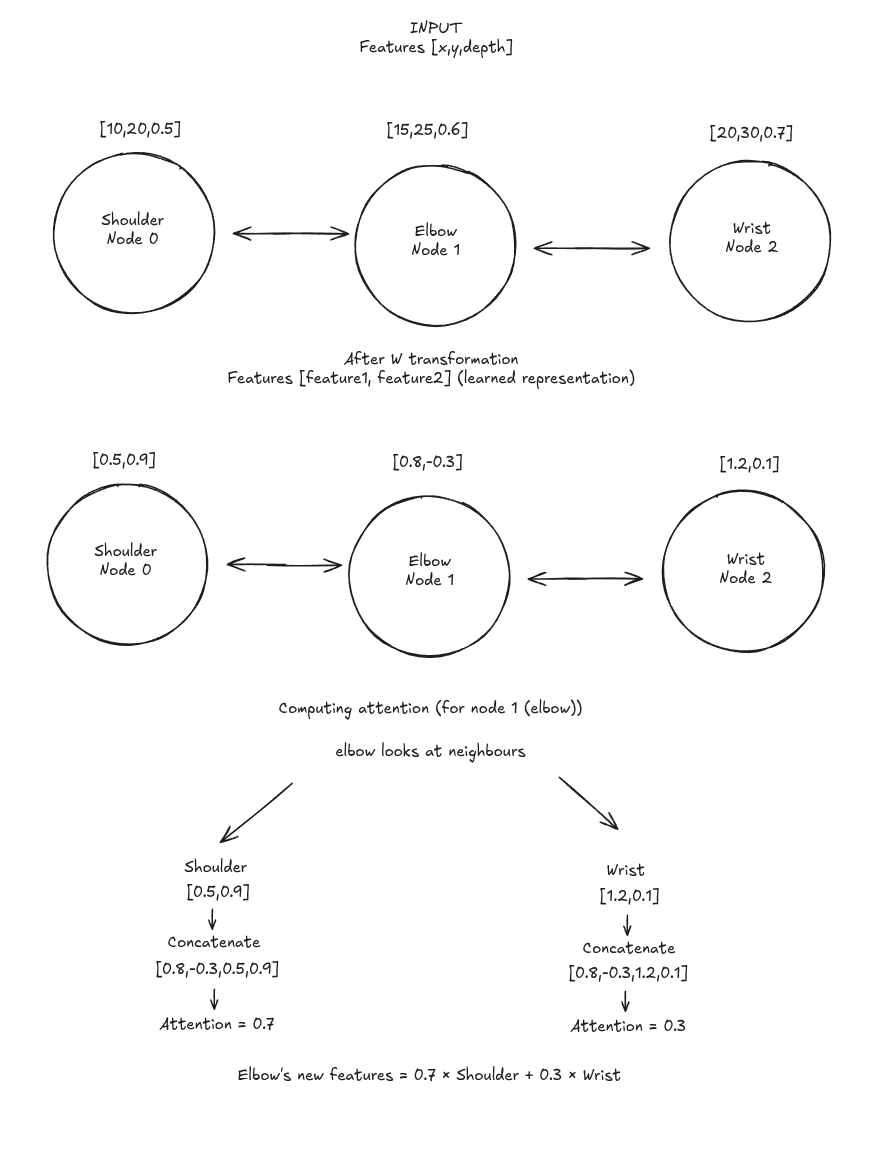
\includegraphics[width=0.4\linewidth]{figures/gat_toy_attention.png}
	\caption{Gat toy example showing how attention is computed between nodes.}
	\label{fig:gat_toy_attention}
\end{figure}

To further explain this simple version of attention the following example is
given computing attention between two nodes, concatenate their features:

\begin{compactitem} 
   \item Node 0 has 2 features (after transformation by $W$)
   \item Node 1 has 2 features (after transformation by $W$) 
   \item Node 2 has 2 features (after transformation by $W$) 
   \item When looking at 2 nodes (neighbours) they are then concatenated: $2 + 2 = 4$ features total 
\end{compactitem}

The $[4 \times 1]$ vector takes these 4 inputs and produces 1 output (the attention score). This is done 
using fake numbers

Say after transformation by $W$ where $W$ is $[3 \times 2]$ matrix
\begin{compactitem}
    \item Shoulder (node 0)  features: $[0.5, 0.9]$
    \item Elbow (node 1)features: $[0.8, -0.3]$
    \item Wrist (node 2) features: $[1.2, 0.1]$
\end{compactitem}

When elbow looks at shoulder:

\begin{enumerate}
    \item Concatenate: $[0.8, -0.3, 0.5, 0.9]$ (4 features)
    \item self.a is like weights: $[w_1, w_2, w_3, w_4]$
    \item Compute: $w_1 \times 0.8 + w_2 \times (-0.3) + w_3 \times 0.5 + w_4 \times 0.9 = \text{attention score}$
    \item After nonlinearity, this might become $0.7$
\end{enumerate}


When elbow looks at wrist:

\begin{enumerate}
    \item Concatenate: $[0.8, -0.3, 1.2, 0.1]$ (4 features)
    \item self.a is like weights: $[w_1, w_2, w_3, w_4]$
    \item Compute: $w_1 \times 0.8 + w_2 \times (-0.3) + w_3 \times 1.2 + w_4 \times 0.1 = \text{attention score}$
    \item After nonlinearity, this might become $0.3$
\end{enumerate}

Initially self.a stores weights like $[[w_1,w_2,w_3,w_4]]$

\begin{lstlisting}[style=pythonstyle,title={Calculating score from concatenated vector},label={code:toy_gat_score}]
   concatenated = [0.8, -0.3, 0.5, 0.9]
   score = self.a(concatenated)
\end{lstlisting}

where the matrix multiplication looks something like this (for elbow looking at shoulder):
\begin{equation}
\label{eq:gat_toy_attention_score}
[w_1, w_2, w_3, w_4] \times 
\begin{bmatrix}
0.8 \\
-0.3 \\
0.5 \\
0.9
\end{bmatrix}
= w_1 \times 0.8 + w_2 \times (-0.3) + w_3 \times 0.5 + w_4 \times 0.9
\end{equation}

The network learns that (looking at the image \ref{fig:gat_toy_attention}):
\begin{compactitem}
    \item Elbow$\rightarrow$Shoulder connection might be important for understanding arm position (score = $0.7$)
    \item Elbow$\rightarrow$Wrist connection might be less critical (score = $0.3$)
\end{compactitem}

(this is just a silly example since the wrist position would be very important but it's about the underlying idea)

The toy problem can then be build using the following code snippet

\begin{lstlisting}[style=pythonstyle,title={Setting up toy problem},label={code:toy_gat_setup}]
def create_toy_example():
    """
    Create a simple 3-node graph representing:
    Node 0 -- Node 1 -- Node 2
    Like: Shoulder -- Elbow -- Wrist
    """
    # Node features: [x, y, depth] (simplified)
    features = torch.tensor([
        [10.0, 20.0, 0.5],  # Node 0 (shoulder)
        [15.0, 25.0, 0.6],  # Node 1 (elbow)
        [20.0, 30.0, 0.7],  # Node 2 (wrist)
    ], dtype=torch.float32)
    
    # Adjacency matrix (who connects to whom)
    adj = torch.tensor([
        [0, 1, 0],  # Node 0 connects to Node 1
        [1, 0, 1],  # Node 1 connects to Node 0 and 2
        [0, 1, 0],  # Node 2 connects to Node 1
    ], dtype=torch.float32)
    
    return features, adj

def visualize_attention(features, adj, attention):
    """Visualize the graph and attention weights"""
    fig, (ax1, ax2) = plt.subplots(1, 2, figsize=(12, 5))
    
    # Plot 1: Original graph structure
    ax1.set_title("Graph Structure")
    ax1.imshow(adj.numpy(), cmap='Blues', vmin=0, vmax=1)
    ax1.set_xticks([0, 1, 2])
    ax1.set_yticks([0, 1, 2])
    ax1.set_xticklabels(['Node 0', 'Node 1', 'Node 2'])
    ax1.set_yticklabels(['Node 0', 'Node 1', 'Node 2'])
    
    # Add values
    for i in range(3):
        for j in range(3):
            ax1.text(j, i, f'{adj[i,j]:.0f}', ha='center', va='center')
    
    # Plot 2: Attention weights
    ax2.set_title("Learned Attention Weights")
    im = ax2.imshow(attention.detach().numpy(), cmap='Reds', vmin=0, vmax=1)
    ax2.set_xticks([0, 1, 2])
    ax2.set_yticks([0, 1, 2])
    ax2.set_xticklabels(['Node 0', 'Node 1', 'Node 2'])
    ax2.set_yticklabels(['Node 0', 'Node 1', 'Node 2'])
    
    # Add values
    for i in range(3):
        for j in range(3):
            ax2.text(j, i, f'{attention[i,j]:.2f}', ha='center', va='center')
    
    plt.colorbar(im, ax=ax2)
    plt.tight_layout()
    plt.show()
\end{lstlisting}

The exact details aren't going to be covered but it follows on from before.
Create features with the values $[10.0, 20.0, 0.5]$ for node 0, $[15.0, 25.0, 0.6]$ for node 1 and $[20.0, 30.0, 0.7]$ for node 2.
The adjacency matrix is created to represent the connections between the nodes

This can be run with the following main

\begin{lstlisting}[style=pythonstyle,title={Toy GAT main},label={code:toy_gat_main}]
def main():
    print("=== Simple GAT Toy Example ===\n")
    
    features, adj = create_toy_example()
    
    print("Input Features (3 nodes):")
    print("Node 0 (shoulder):", features[0].numpy())
    print("Node 1 (elbow):", features[1].numpy())
    print("Node 2 (wrist):", features[2].numpy())
    
    print("\nAdjacency Matrix:")
    print(adj.numpy())
    print("(1 = connected, 0 = not connected)")
    
    model = SimpleGAT(in_features=3, out_features=2)
    
    output, attention = model(features, adj)
    
    print("\n=== After GAT Processing ===")
    print("\nOutput Features (transformed):")
    for i in range(3):
        print(f"Node {i}:", output[i].detach().numpy())
    
    print("\nAttention Weights (who pays attention to whom):")
    for i in range(3):
        print(f"Node {i} attention:", attention[i].detach().numpy())
    
    visualize_attention(features, adj, attention)
    
    print("\n=== Detailed look at Node 1 (elbow) ===")
    print("Node 1 can see: Node 0 (shoulder) and Node 2 (wrist)")
    print(f"Attention to Node 0: {attention[1, 0]:.3f}")
    print(f"Attention to Node 2: {attention[1, 2]:.3f}")
    print("(These sum to 1.0)")
    
    weighted_sum = (attention[1, 0] * model.W(features[0]) + 
                   attention[1, 2] * model.W(features[2]))
    print(f"\nNode 1's output is weighted sum of its neighbors' transformed features")
    print(weighted_sum)

if __name__ == "__main__":
    main()
\end{lstlisting}

which will produce the following output

\begin{lstlisting}[style=bashstyle,title={Toy GAT main output},label={code:toy_gat_main_output}]
=== Simple GAT Toy Example ===

Input Features (3 nodes):
Node 0 (shoulder): [10.  20.   0.5]
Node 1 (elbow): [15.  25.   0.6]
Node 2 (wrist): [20.  30.   0.7]

Adjacency Matrix:
[[0. 1. 0.]
 [1. 0. 1.]
 [0. 1. 0.]]
(1 = connected, 0 = not connected)

=== After GAT Processing ===

Output Features (transformed):
Node 0: [-5.649103  5.94354 ]
Node 1: [-5.658541   5.9492426]
Node 2: [-5.649103  5.94354 ]

Attention Weights (who pays attention to whom):
Node 0 attention: [0. 1. 0.]
Node 1 attention: [0.49696022 0.         0.5030397 ]
Node 2 attention: [0. 1. 0.]

=== Detailed look at Node 1 (elbow) ===
Node 1 can see: Node 0 (shoulder) and Node 2 (wrist)
Attention to Node 0: 0.497
Attention to Node 2: 0.503
(These sum to 1.0)

Node 1's output is weighted sum of its neighbors' transformed features
tensor([-5.6585,  5.9492], grad_fn=<AddBackward0>)
\end{lstlisting}

where the attention weights are visualized by 

\begin{figure}[H]
	\centering
	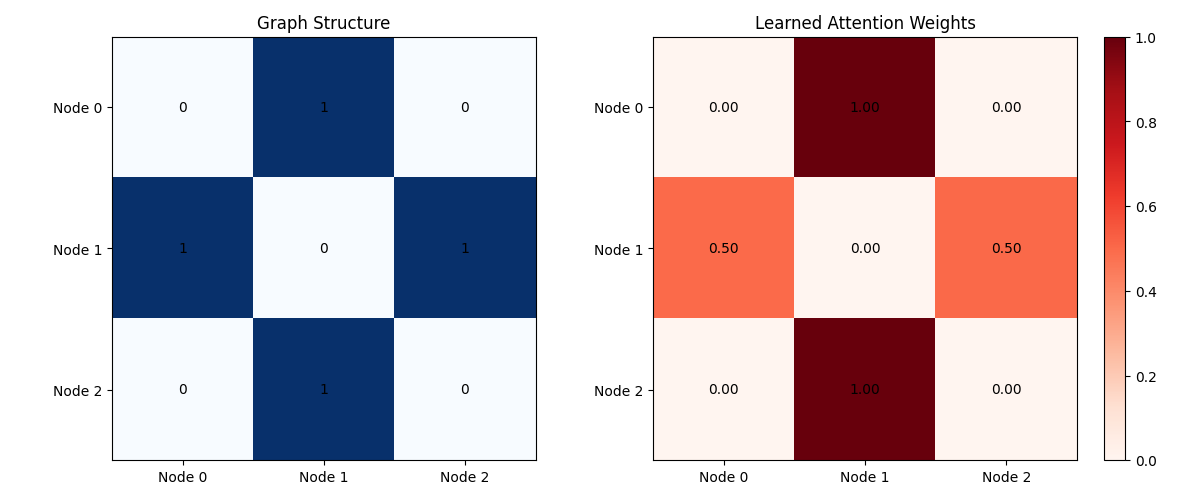
\includegraphics[width=0.8\linewidth]{figures/toy_learned_attention_weights.png}
	\caption{Gat toy example attention weights visualized after running \ref{code:toy_gat_main}}
	\label{fig:gat_toy_attention_vizualized}
\end{figure}

Before I do dummy training I didn't actually explain the forward pass of this GAT

\begin{lstlisting}[style=pythonstyle,title={Toy problem forward pass},label={code:toy_problem_forward_pass}]
def forward(self, features, adj):
    # Step 1: Transform features
    h = self.W(features)  # [N, out_features]
    N = h.size(0)
    
    # Step 2: Prepare for attention computation
    h_i = h.unsqueeze(1).repeat(1, N, 1)  # [N, N, out_features]
    h_j = h.unsqueeze(0).repeat(N, 1, 1)  # [N, N, out_features]
    
    # Step 3: Concatenate pairs
    pairs = torch.cat([h_i, h_j], dim=2)  # [N, N, 2*out_features]
    
    # Step 4: Compute attention scores
    e = F.leaky_relu(self.a(pairs).squeeze(2))  # [N, N]
    
    # Step 5: Mask with adjacency
    mask = -1e9 * (1.0 - adj)
    masked_e = e + mask
    
    # Step 6: Apply softmax
    attention = F.softmax(masked_e, dim=1)
    
    # Step 7: Aggregate features
    output = torch.matmul(attention, h)
    
    return output, attention
\end{lstlisting}

\textbf{Step 1:} Transform the input features

\begin{lstlisting}[style=pythonstyle,title={Toy problem forward pass step 1},label={code:toy_problem_forward_pass_step_1}]
h = self.W(features)  # [N, out_features]
\end{lstlisting}

In this case $h$ is the "hidden" representation of the nodes; $N=3$ and $out\_features=2$ so $h$ will be $[3, 2]$ matrix.

In this example Input = $[[10, 20, 0.5], [15, 25, 0.6], [20, 30, 0.7]]$ and h
(example values) = $[[0.5, 0.9], [0.8, -0.3], [1.2, 0.1]]$

\textbf{Step 2:} Create all pairs 

\begin{lstlisting}[style=pythonstyle,title={Toy problem forward pass step 2},label={code:toy_problem_forward_pass_step_2}]
h_i = h.unsqueeze(1).repeat(1, N, 1)  # [N, N, out_features]
h_j = h.unsqueeze(0).repeat(N, 1, 1)  # [N, N, out_features]
\end{lstlisting}

The goal is to create two tensors where each node's features so that any pair of nodes can be compared

The "from" nodes h\_i (who is looking i.e elbow looking at shoulder and wrist):

\begin{compactitem}
   \item h.unsqueeze(1) adds a dimension: [3,2] → [3,1,2]
   \item .repeat(1, N, 1) repeats along dim 1: [3,1,2] → [3,3,2] 
\end{compactitem}

The "to" nodes h\_j (who is being looked at):

\begin{compactitem}
   \item h.unsqueeze(0) adds a dimension: [3,2] → [1,3,2]
   \item .repeat(N, 1, 1) repeats along dim 0: [1,3,2] → [3,3,2]
\end{compactitem}

Compute attention scores for ALL possible pairs of nodes. To do this
efficiently, it's required to arrange the data so that any pair can be accessed $(i,j)$.

Think of it as a Table

Imagine filling out this attention table:

\begin{center}
\begin{tabular}{c|c|c|c}
 & \multicolumn{3}{c}{Who is being looked at (j)} \\
 & Node 0 & Node 1 & Node 2 \\
\hline
\multirow{3}{*}{\rotatebox{90}{Who is looking (i)}} 
Node 0 & $0 \rightarrow 0$ & $0 \rightarrow 1$ & $0 \rightarrow 2$ \\
Node 1 & $1 \rightarrow 0$ & $1 \rightarrow 1$ & $1 \rightarrow 2$ \\
Node 2 & $2 \rightarrow 0$ & $2 \rightarrow 1$ & $2 \rightarrow 2$ \\
\end{tabular}
\end{center}

Each cell $(i,j)$ represents ``node $i$ attending to node $j$''

What $h_i$ and $h_j$ Do

\textbf{$h_i$ stores the ``looker's'' features:}
\begin{compactitem}
    \item At position $[0,0], [0,1], [0,2] \rightarrow$ Node 0's features
    \item At position $[1,0], [1,1], [1,2] \rightarrow$ Node 1's features
    \item At position $[2,0], [2,1], [2,2] \rightarrow$ Node 2's features
\end{compactitem}

\textbf{$h_j$ stores the ``looked at'' features:}
\begin{compactitem}
    \item At position $[0,0], [1,0], [2,0] \rightarrow$ Node 0's features
    \item At position $[0,1], [1,1], [2,1] \rightarrow$ Node 1's features
    \item At position $[0,2], [1,2], [2,2] \rightarrow$ Node 2's features
\end{compactitem}

Fill in the table with actual features:

\begin{center}
\textbf{$h_i$ (looker's features):}
\begin{tabular}{c|c|c|c}
 & $j=0$ & $j=1$ & $j=2$ \\
\hline
$i=0$ & $[0.5,0.9]$ & $[0.5,0.9]$ & $[0.5,0.9]$ \\
$i=1$ & $[0.8,-0.3]$ & $[0.8,-0.3]$ & $[0.8,-0.3]$ \\
$i=2$ & $[1.2,0.1]$ & $[1.2,0.1]$ & $[1.2,0.1]$ \\
\end{tabular}
\end{center}

\begin{center}
\textbf{$h_j$ (looked at features):}
\begin{tabular}{c|c|c|c}
 & $j=0$ & $j=1$ & $j=2$ \\
\hline
$i=0$ & $[0.5,0.9]$ & $[0.8,-0.3]$ & $[1.2,0.1]$ \\
$i=1$ & $[0.5,0.9]$ & $[0.8,-0.3]$ & $[1.2,0.1]$ \\
$i=2$ & $[0.5,0.9]$ & $[0.8,-0.3]$ & $[1.2,0.1]$ \\
\end{tabular}
\end{center}

Specific Example: Position $[1,0]$

At position $[1,0]$ (row 1, column 0):
\begin{compactitem}
    \item This means ``Node 1 looking at Node 0''
    \item $h_i[1,0] = [0.8, -0.3]$ $\leftarrow$ Node 1's features (the looker)
    \item $h_j[1,0] = [0.5, 0.9]$ $\leftarrow$ Node 0's features (being looked at)
\end{compactitem}

\textbf{Step 3:} Concatenate pairs

\begin{compactitem}
    \item $\text{pairs}[1,0] = [0.8, -0.3, 0.5, 0.9]$
    \item This represents: [Elbow features, Shoulder features]
\end{compactitem}

The attention mechanism will use this concatenated vector to decide how much
the elbow should pay attention to the shoulder!

Position $[i,j]$ = $[features\_of\_i, features\_of\_j]$:

As an example:

pairs[1,0] = [0.8, -0.3, 0.5, 0.9]  (Elbow looking at Shoulder)

pairs[1,2] = [0.8, -0.3, 1.2, 0.1]  (Elbow looking at Wrist)

\textbf{Step 4:} Compute Attention Scores 

$e = F.leaky\_relu(self.a(pairs).squeeze(2))  [N, N]$

where in this case $e[i,j]$ is the attention score for node $i$ looking at node $j$.

\textbf{Step 5:} Mask with adjacency

\begin{lstlisting}[style=pythonstyle,title={Toy problem forward pass step 5},label={code:toy_problem_forward_pass_step_5}]
mask = -1e9 * (1.0 - adj)
masked_e = e + mask
\end{lstlisting}

This is a crucial step to ensure that nodes only pay attention to their neighbors.

Basically if:

adj[i,j] = 0 (no connection), then masked\_e[i,j] = -inf (no attention)

if adj[i,j] = 1 (connected), then masked\_e[i,j] = e[i,j] (keep attention score)


\textbf{Step 6:} Apply softmax

$attention = F.softmax(masked\_e, dim=1)$

Softmax turns scores into probabilities:

Very negative values (-1e9) become approximately 0

Connected nodes get normalized attention weights that sum to 1

For node 1 (elbow):

Before softmax: [some\_value, -1e9, some\_value]

After softmax: [0.497, 0.0, 0.503]

\textbf{Step 7:} Aggregate Features

$output = torch.matmul(attention, h)$

Each node's output is a weighted sum of its neighbors' transformed features:

For node 1:

\begin{align}
\label{eq:gat_toy_output}
\text{output}[1] &= 0.497 \cdot h[0] + 0.0 \cdot h[1] + 0.503 \cdot h[2] \notag \\
                 &= 0.497 \cdot [0.5, 0.9] + 0.503 \cdot [1.2, 0.1] \notag \\
                 &= [0.85, 0.50] \quad \text{(approximately)}
\end{align}


While this is a toy problem extend it to training given dummy targets as well
to see how this will ultimately work

This is a full example of simple GAT, setting up the problem and training. I'll
exaplain some parts after the code

\begin{lstlisting}[style=pythonstyle,title={Toy problem with fake training},label={code:toy_problem_with_fake_training}]
import torch
import torch.nn as nn
import torch.nn.functional as F
import matplotlib.pyplot as plt
import numpy as np

class SimpleGAT(nn.Module):
    def __init__(self, in_features, out_features):
        super(SimpleGAT, self).__init__()
        self.W = nn.Linear(in_features, out_features, bias=False)
        self.a = nn.Linear(2 * out_features, 1, bias=False)
        
    def forward(self, features, adj):
        h = self.W(features)
        N = h.size(0)
        
        h_i = h.unsqueeze(1).repeat(1, N, 1)
        h_j = h.unsqueeze(0).repeat(N, 1, 1)
        
        pairs = torch.cat([h_i, h_j], dim=2)
        e = F.leaky_relu(self.a(pairs).squeeze(2))
        
        mask = -1e9 * (1.0 - adj)
        masked_e = e + mask
        
        attention = F.softmax(masked_e, dim=1)
        output = torch.matmul(attention, h)
        
        return output, attention

def create_toy_data_with_targets():
    """
    Create toy data with made-up target outputs
    The network to learn to output 
    specific features based on the node position
    """
    # Input features: [x, y, depth]
    features = torch.tensor([
        [10.0, 20.0, 0.5],  # Shoulder
        [15.0, 25.0, 0.6],  # Elbow
        [20.0, 30.0, 0.7],  # Wrist
    ], dtype=torch.float32)
    
    # Adjacency matrix
    adj = torch.tensor([
        [0, 1, 0],
        [1, 0, 1],
        [0, 1, 0],
    ], dtype=torch.float32)
    
    # Made-up target outputs: 
    # [forward_reach, upward_reach] for each joint
    targets = torch.tensor([
        [0.3, 0.8],  # Shoulder: low forward, high upward
        [0.6, 0.5],  # Elbow: medium both
        [0.9, 0.2],  # Wrist: high forward, low upward
    ], dtype=torch.float32)
    
    return features, adj, targets

def train_toy_gat(num_epochs=100):
    """
    Train the toy GAT model
    """
    # Create data
    features, adj, targets = create_toy_data_with_targets()
    
    # Initialize model
    model = SimpleGAT(in_features=3, out_features=2)
    
    # Loss and optimizer
    criterion = nn.MSELoss()
    optimizer = torch.optim.Adam(model.parameters(), lr=0.01)
    
    # Training history
    losses = []
    
    print("=== Training Toy GAT ===\n")
    print("Target outputs want to learn:")
    print("Shoulder:", targets[0].numpy(), "(low forward, high upward)")
    print("Elbow:", targets[1].numpy(), "(medium both)")
    print("Wrist:", targets[2].numpy(), "(high forward, low upward)")
    print("\nStarting training...")
    
    for epoch in range(num_epochs):
        # Forward pass
        output, attention = model(features, adj)
        
        # Compute loss
        loss = criterion(output, targets)
        
        # Backward pass
        optimizer.zero_grad()
        loss.backward()
        optimizer.step()
        
        # Record loss
        losses.append(loss.item())
        
        # Print progress
        if epoch % 10 == 0:
            print(f"Epoch {epoch:3d}, Loss: {loss.item():.4f}")
    
    print("\n=== Training Complete ===")
    
    # Final predictions
    model.eval()
    with torch.no_grad():
        final_output, final_attention = model(features, adj)
    
    print("\nFinal predictions vs targets:")
    for i, joint in enumerate(['Shoulder', 'Elbow', 'Wrist']):
        pred = final_output[i].numpy()
        targ = targets[i].numpy()
        print(f"{joint}: Predicted {pred}, Target {targ}")
    
    print("\nFinal attention weights:")
    print(final_attention.numpy())
    
    # Plot training loss
    plt.figure(figsize=(10, 4))
    
    plt.subplot(1, 2, 1)
    plt.plot(losses)
    plt.title('Training Loss')
    plt.xlabel('Epoch')
    plt.ylabel('MSE Loss')
    
    # Plot final attention
    plt.subplot(1, 2, 2)
    plt.imshow(final_attention.detach().numpy(), cmap='Reds', vmin=0, vmax=1)
    plt.colorbar()
    plt.title('Final Attention Weights')
    plt.xticks([0, 1, 2], ['Shoulder', 'Elbow', 'Wrist'])
    plt.yticks([0, 1, 2], ['Shoulder', 'Elbow', 'Wrist'])
    
    # Add values
    for i in range(3):
        for j in range(3):
            plt.text(j, i, f'{final_attention[i,j]:.2f}', 
                    ha='center', va='center')
    
    plt.tight_layout()
    plt.show()
    
    return model, losses

def analyze_what_gat_learned(model, features, adj):
    """
    Analyze what the GAT learned during training
    """
    print("\n=== Analyzing What GAT Learned ===\n")
    
    # Get the learned weights
    W_weights = model.W.weight.data.numpy()
    a_weights = model.a.weight.data.numpy()
    
    print("Learned transformation matrix W:")
    print(W_weights)
    print("\nThis transforms [x, y, depth] -> [feature1, feature2]")
    
    print("\nLearned attention weights a:")
    print(a_weights)
    print("\nThis computes importance of node pairs")
    
    # Show how each node's features are transformed
    with torch.no_grad():
        transformed = model.W(features)
        
    print("\nHow each node's features are transformed:")
    for i, joint in enumerate(['Shoulder', 'Elbow', 'Wrist']):
        orig = features[i].numpy()
        trans = transformed[i].numpy()
        print(f"{joint}: {orig} -> {trans}")

if __name__ == "__main__":
    # Train the model
    model, losses = train_toy_gat(num_epochs=100)
    
    # Analyze what was learned
    features, adj, _ = create_toy_data_with_targets()
    analyze_what_gat_learned(model, features, adj)
\end{lstlisting}

The SimpleGat remains the same as before.

Create toy target is mostly the same but it has targets (specific features
based on the node posiition) in this case the targets are [forward\_reach,
upward\_reach] so the shoulder being [0.3,0.8] is low forward and high upward

The train toy gat function is given 

\begin{lstlisting}[style=pythonstyle,title={Train toy gat function},label={code:train_toy_gat}]
def train_toy_gat(num_epochs=100):
    """
    Train the toy GAT model
    """
    # Create data
    features, adj, targets = create_toy_data_with_targets()
    
    # Initialize model
    model = SimpleGAT(in_features=3, out_features=2)
    
    # Loss and optimizer
    criterion = nn.MSELoss()
    optimizer = torch.optim.Adam(model.parameters(), lr=0.01)
    
    # Training history
    losses = []
    
    print("=== Training Toy GAT ===\n")
    print("Target outputs want to learn:")
    print("Shoulder:", targets[0].numpy(), "(low forward, high upward)")
    print("Elbow:", targets[1].numpy(), "(medium both)")
    print("Wrist:", targets[2].numpy(), "(high forward, low upward)")
    print("\nStarting training...")
    
    for epoch in range(num_epochs):
        # Forward pass
        output, attention = model(features, adj)
        
        # Compute loss
        loss = criterion(output, targets)
        
        # Backward pass
        optimizer.zero_grad()
        loss.backward()
        optimizer.step()
        
        # Record loss
        losses.append(loss.item())
        
        # Print progress
        if epoch % 10 == 0:
            print(f"Epoch {epoch:3d}, Loss: {loss.item():.4f}")
    
    print("\n=== Training Complete ===")
    
    # Final predictions
    model.eval()
    with torch.no_grad():
        final_output, final_attention = model(features, adj)
    
    print("\nFinal predictions vs targets:")
    for i, joint in enumerate(['Shoulder', 'Elbow', 'Wrist']):
        pred = final_output[i].numpy()
        targ = targets[i].numpy()
        print(f"{joint}: Predicted {pred}, Target {targ}")
    
    print("\nFinal attention weights:")
    print(final_attention.numpy())
    
    # Plot training loss
    plt.figure(figsize=(10, 4))
    
    plt.subplot(1, 2, 1)
    plt.plot(losses)
    plt.title('Training Loss')
    plt.xlabel('Epoch')
    plt.ylabel('MSE Loss')
    
    # Plot final attention
    plt.subplot(1, 2, 2)
    plt.imshow(final_attention.detach().numpy(), cmap='Reds', vmin=0, vmax=1)
    plt.colorbar()
    plt.title('Final Attention Weights')
    plt.xticks([0, 1, 2], ['Shoulder', 'Elbow', 'Wrist'])
    plt.yticks([0, 1, 2], ['Shoulder', 'Elbow', 'Wrist'])
    
    # Add values
    for i in range(3):
        for j in range(3):
            plt.text(j, i, f'{final_attention[i,j]:.2f}', 
                    ha='center', va='center')
    
    plt.tight_layout()
    plt.show()
    
    return model, losses
\end{lstlisting}

\textbf{Training Process Overview}

The training function demonstrates how GAT learns to produce target outputs through iterative optimization.

Training Setup:

The function initializes:

\begin{compactitem}
   \item \textbf{Model}: SimpleGAT with 3 input features and 2 output features
   \item \textbf{Loss function}: Mean Squared Error (MSE) to measure prediction error
   \item \textbf{Optimizer}: Adam with learning rate 0.01 for updating model parameters
   \item \textbf{Target outputs}: [forward\_reach, upward\_reach] for each joint
      \begin{compactitem}
         \item Shoulder: [0.3, 0.8] (low forward, high upward)
         \item Elbow: [0.6, 0.5] (medium both)
         \item Wrist: [0.9, 0.2] (high forward, low upward)
      \end{compactitem}
\end{compactitem}

Training Loop Steps: 

For each epoch, the following steps occur:

\textbf{1. Forward Pass}

\begin{lstlisting}[style=pythonstyle]
output, attention = model(features, adj)
\end{lstlisting}

The model processes the graph and produces:
\begin{compactitem}
   \item \texttt{output}: Predicted features for each node [3, 2]
   \item \texttt{attention}: Learned attention weights [3, 3]
\end{compactitem}

\textbf{2. Loss Computation}

\begin{lstlisting}[style=pythonstyle]
loss = criterion(output, targets)
\end{lstlisting}

MSE loss calculates the average squared difference between predictions and targets:

\begin{equation}
   \label{eq:mse_loss}   
   \text{MSE} = \frac{1}{N} \sum_{i=1}^{N} (\text{output}_i - \text{target}_i)^2
\end{equation}

\textbf{3. Backward Pass}

\begin{lstlisting}[style=pythonstyle]
optimizer.zero_grad()
loss.backward()
optimizer.step()
\end{lstlisting}

This sequence:
\begin{compactitem}
   \item Clears previous gradients
   \item Computes gradients via backpropagation
   \item Updates model parameters (W and a) based on gradients
\end{compactitem}

Learning Process

During training, the model learns:

\begin{compactitem}
   \item \textbf{Transformation matrix W}: How to convert [x, y, depth] into meaningful features
   \item \textbf{Attention weights a}: Which connections are important for predicting targets
\end{compactitem}

The attention mechanism discovers which neighbors provide useful information.
For example, if predicting forward reach requires information from adjacent
joints, the model learns to increase attention weights for those connections.

Evaluation:

After training completes:
\begin{lstlisting}[style=pythonstyle]
model.eval()
with torch.no_grad():
   final_output, final_attention = model(features, adj)
\end{lstlisting}

The model is set to evaluation mode and final predictions are made without gradient computation. The results show:

\begin{compactitem}
   \item How close predictions are to targets
   \item Final learned attention patterns
   \item Training loss curve showing convergence
\end{compactitem}

and can be visualized as seen below

\begin{figure}[H]
	\centering
	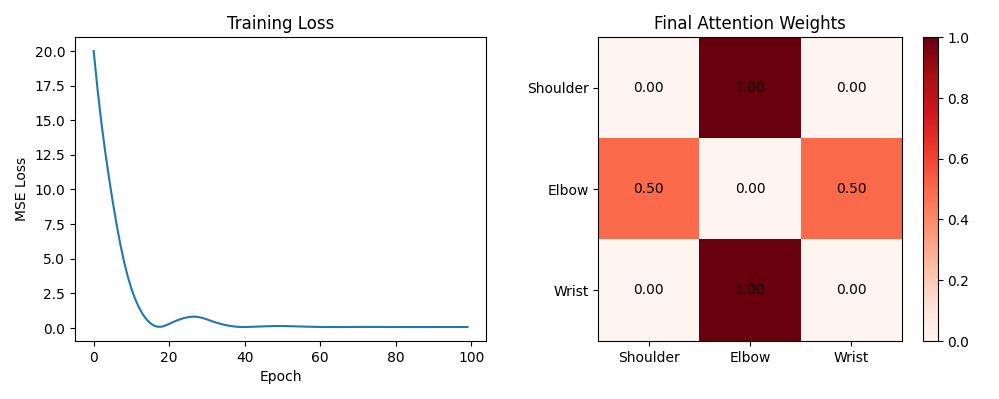
\includegraphics[width=0.8\linewidth]{figures/gat_toy_trained.png}
	\caption{Gat toy example training and attention weights visualized}
	\label{fig:gat_toy_trained}
\end{figure}

and the terminal output given as

\begin{lstlisting}[style=bashstyle,title={Toy GAT training output},label={code:toy_gat_trained_output}]
=== Training Toy GAT ===

Target outputs want to learn:
Shoulder: [0.3 0.8] (low forward, high upward)
Elbow: [0.6 0.5] (medium both)
Wrist: [0.9 0.2] (high forward, low upward)

Starting training...
Epoch   0, Loss: 20.0001
Epoch  10, Loss: 2.8260
Epoch  20, Loss: 0.2882
Epoch  30, Loss: 0.6119
Epoch  40, Loss: 0.0604
Epoch  50, Loss: 0.1305
Epoch  60, Loss: 0.0659
Epoch  70, Loss: 0.0663
Epoch  80, Loss: 0.0617
Epoch  90, Loss: 0.0606

=== Training Complete ===

Final predictions vs targets:
Shoulder: Predicted [0.62246007 0.5006373 ], Target [0.3 0.8]
Elbow: Predicted [0.6203502  0.49830887], Target [0.6 0.5]
Wrist: Predicted [0.62246007 0.5006373 ], Target [0.9 0.2]

Final attention weights:
[[0.        1.        0.       ]
 [0.4988925 0.        0.5011075]
 [0.        1.        0.       ]]

=== Analyzing What GAT Learned ===

Learned transformation matrix W:
[[-0.5457222   0.3693933  -0.7108979 ]
 [-0.5797511   0.37739122 -0.39646104]]

This transforms [x, y, depth] -> [feature1, feature2]

Learned attention weights a:
[[-0.25833952 -0.02046523 -0.15695873 -0.06844266]]

This computes importance of node pairs

How each node's features are transformed:
Shoulder: [10.  20.   0.5] -> [1.5751951 1.5520833]
Elbow: [15.  25.   0.6] -> [0.62246007 0.5006373 ]
Wrist: [20.  30.   0.7] -> [-0.33027396 -0.5508076 ]
\end{lstlisting}

\subsection{Graph Attention Network (GAT)}

This is the entire file and again I'll break it down

\begin{lstlisting}[style=pythonstyle,title={Basic Gat Code},label={code:basic_gat}]
import torch
import torch.nn as nn
import torch.nn.functional as F
import numpy as np

class GraphAttentionLayer(nn.Module):
    """
    Simple Graph Attention Layer
    """
    def __init__(self, in_features, out_features, dropout=0.6, alpha=0.2):
        super(GraphAttentionLayer, self).__init__()
        self.in_features = in_features
        self.out_features = out_features
        self.dropout = dropout
        self.alpha = alpha
        
        # Linear transformation for node features
        self.W = nn.Linear(in_features, out_features, bias=False)
        
        # Attention mechanism parameters
        self.a = nn.Linear(2 * out_features, 1, bias=False)
        
        # LeakyReLU for attention
        self.leakyrelu = nn.LeakyReLU(self.alpha)
        
        self.reset_parameters()
    
    def reset_parameters(self):
        nn.init.xavier_uniform_(self.W.weight)
        nn.init.xavier_uniform_(self.a.weight)
    
    def forward(self, features, adj):
        """
        Args:
            features: Node features [N, in_features]
            adj: Adjacency matrix [N, N]
        Returns:
            Updated node features [N, out_features]
        """
        N = features.size(0)
        
        # Apply linear transformation
        h = self.W(features)  # [N, out_features]
        
        # Self-attention on nodes
        a_input = self._prepare_attention_input(h)  # [N, N, 2*out_features]
        e = self.leakyrelu(self.a(a_input).squeeze(2))  # [N, N]
        
        # Mask attention scores using adjacency matrix
        zero_vec = -9e15 * torch.ones_like(e)
        attention = torch.where(adj > 0, e, zero_vec)  # [N, N]
        
        # Apply softmax
        attention = F.softmax(attention, dim=1)
        attention = F.dropout(attention, self.dropout, training=self.training)
        
        # Apply attention to features
        h_prime = torch.matmul(attention, h)  # [N, out_features]
        
        return h_prime
    
    def _prepare_attention_input(self, h):
        """
        Prepare input for attention mechanism
        """
        N = h.size(0)
        
        # Repeat h1 and h2 to create all pairs
        h_repeat = h.repeat(N, 1).view(N, N, -1)  # [N, N, out_features]
        h_repeat_interleave = h.repeat_interleave(N, dim=0).view(N, N, -1)  # [N, N, out_features]
        
        # Concatenate them
        a_input = torch.cat([h_repeat_interleave, h_repeat], dim=-1)  # [N, N, 2*out_features]
        
        return a_input


class DepthAwareGAT(nn.Module):
    """
    Depth-Aware Graph Attention Network for pose estimation
    """
    def __init__(self, input_dim, hidden_dim=64, output_dim=32, num_heads=4, dropout=0.6):
        super(DepthAwareGAT, self).__init__()
        
        self.input_dim = input_dim
        self.hidden_dim = hidden_dim
        self.output_dim = output_dim
        self.num_heads = num_heads
        self.dropout = dropout
        
        # Multi-head attention layers
        self.attention_heads = nn.ModuleList([
            GraphAttentionLayer(input_dim, hidden_dim, dropout=dropout)
            for _ in range(num_heads)
        ])
        
        # Output layer
        self.out_attention = GraphAttentionLayer(
            hidden_dim * num_heads, 
            output_dim, 
            dropout=dropout
        )
        
        # Additional layers for task-specific outputs
        self.mlp = nn.Sequential(
            nn.Linear(output_dim, output_dim),
            nn.ReLU(),
            nn.Dropout(dropout),
            nn.Linear(output_dim, output_dim)
        )
        
    def forward(self, node_features, adj_matrix):
        """
        Forward pass through the GAT
        
        Args:
            node_features: Node features [N, input_dim]
            adj_matrix: Adjacency matrix [N, N]
            
        Returns:
            output: Processed node features [N, output_dim]
        """
        # Apply dropout to input
        x = F.dropout(node_features, self.dropout, training=self.training)
        
        # Multi-head attention
        head_outputs = []
        for attention_head in self.attention_heads:
            head_output = attention_head(x, adj_matrix)
            head_outputs.append(head_output)
        
        # Concatenate all heads
        x = torch.cat(head_outputs, dim=1)  # [N, hidden_dim * num_heads]
        x = F.elu(x)
        x = F.dropout(x, self.dropout, training=self.training)
        
        # Final attention layer
        x = self.out_attention(x, adj_matrix)  # [N, output_dim]
        x = F.elu(x)
        
        # Task-specific processing
        output = self.mlp(x)
        
        return output
    
    def compute_graph_embedding(self, node_features, adj_matrix):
        """
        Compute a single embedding for the entire graph
        
        Args:
            node_features: Node features [N, input_dim]
            adj_matrix: Adjacency matrix [N, N]
            
        Returns:
            graph_embedding: Graph-level embedding [output_dim]
        """
        # Get node embeddings
        node_embeddings = self.forward(node_features, adj_matrix)
        
        # Simple mean pooling
        graph_embedding = torch.mean(node_embeddings, dim=0)
        
        return graph_embedding
\end{lstlisting}

\subsubsection{GAT Overview}
The GAT implementation has two main components:

1. GraphAttentionLayer (Single Attention Layer)

This is the building block that implements the graph attention mechanism:

\begin{compactitem}
   \item Takes node features and adjacency matrix
   \item Learns which neighbors are important (attention weights)
   \item Aggregates information from neighbors based on learned importance
   \item Only attends to connected nodes (uses adjacency matrix as mask)
\end{compactitem}

2. DepthAwareGAT (Complete Model)

This is the full model that:

\begin{compactitem}
   \item Multiple GraphAttentionLayers in parallel (multi-head attention)
   \item Stacks layers for deeper processing
   \item Outputs refined node embeddings 
   \item Can produce graph-level embeddings via pooling
\end{compactitem}

The Flow:

\begin{compactitem}
   \item Input: Nodes with features $[x, y, depth, confidence, joint\_embedding]$
   \item Multi-head Attention: 4 parallel attention heads learn different aspects
   \item Concatenation: Combine all head outputs
   \item Final Attention: One more attention layer to refine
   \item MLP: Task-specific processing
   \item Output: Refined embeddings for each node
\end{compactitem}

Key Concepts:

\begin{compactitem}
   \item Attention: Learn which connected joints matter most for each joint
   \item Multi-head: Like having 4 different "experts" looking at the pose
   \item Masking: Only look at anatomically connected joints (via adjacency)
   \item Depth-aware: Incorporates 3D information through the depth features
\end{compactitem}

The model essentially learns to refine each joint's representation by
intelligently aggregating information from its connected neighbors, considering
both 2D position and depth.
